
\documentclass[12pt]{article}

%\usepackage[pdf]{pstricks}
%\usepackage[on]{auto-pst-pdf}

\topmargin 0in
\oddsidemargin 0.25in
\evensidemargin 0.25in
\textwidth 6.0in
\textheight 9.0in

%FXG Math Macros
\usepackage[english]{babel} 
%\usepackage{algorithm}
%\usepackage{algorithm2e}

%\usepackage[numbered]{algo}
%\usepackage{pseudocode}

%\usepackage{algorithmic}
%\usepackage{algorithmicx}
%\usepackage{algpseudocode}

\usepackage{epsfig}

%\usepackage[chapter]{algorithm}
\usepackage{algorithmicx}
\usepackage{algpseudocode}

\usepackage{subfigure}
\usepackage{stmaryrd}
\usepackage{amsmath} 
\usepackage{color}
\usepackage{amssymb} 
\usepackage{amsfonts} 

%\usepackage[dvips]{graphicx} 

%\usepackage{floatflt} 
\usepackage{mathrsfs}
%\usepackage{mathabx}
%\usepackage{wasysym} 
%\usepackage{showkeys}

\usepackage[T1]{fontenc}
\usepackage[utf8]{inputenc}
\usepackage[font=small,labelfont=bf,tableposition=top]{caption}
%\usepackage[font=footnotesize]{subcaption}
\usepackage{multicol}

\usepackage{float}
\usepackage{graphicx}
\input{epsf}

\newtheorem{theorem}{Theorem}
\newtheorem{acknowledgement}[theorem]{Acknowledgement}
%\newtheorem{algorithm}[theorem]{Algorithm}
\newtheorem{axiom}[theorem]{Axiom}
\newtheorem{case}[theorem]{Case}
\newtheorem{claim}[theorem]{Claim}
\newtheorem{conclusion}[theorem]{Conclusion}
\newtheorem{condition}[theorem]{Condition}
\newtheorem{conjecture}[theorem]{Conjecture}
\newtheorem{corollary}[theorem]{Corollary}
\newtheorem{criterion}[theorem]{Criterion}
\newtheorem{definition}[theorem]{Definition}
\newtheorem{example}[theorem]{Example}
\newtheorem{exercise}[theorem]{Exercise}
\newtheorem{lemma}[theorem]{Lemma}
\newtheorem{notation}[theorem]{Notation}
\newtheorem{problem}[theorem]{Problem}
\newtheorem{proposition}[theorem]{Proposition}
\newtheorem{remark}[theorem]{Remark}
\newtheorem{solution}[theorem]{Solution}
\newtheorem{summary}[theorem]{Summary}
\newenvironment{proof}[1][Proof]{\textbf{#1.} }{\ \rule{0.5em}{0.5em}}
%\newenvironment{homework}[1][Homework]{\textbf{#1.} }{\ \rule{0.5em}{0.5em}}
%\newtheorem{homework}[theorem]{Exercise}
%\newtheorem{homework}[section]{Exercise}
\newtheorem{homework}[subsubsection]{Exercise}
%\newtheorem{remark}[section]{Remark}
%\input{tcilatex}

%FXG Commands
\newtheorem{guess}{Definition}
\newcommand{\comment}[1] {}
\newcommand{\Norder} {N}
\newcommand{\order}{\mathcal{O}}
\newcommand{\Npoints} {N_p}
\newcommand{\Nfaces} {N_{f}}
\newcommand{\Nelements} {N_e}

\newcommand{\Dweak}{\wt{D}}
\newcommand{\diff}[2] {\frac{\partial #1}{\partial #2}}
\newcommand{\dxx}[2] {\frac{\partial^2 #1}{\partial {#2}^2}}
\newcommand{\difft}[2] {\frac{d #1}{d #2}}
\newcommand{\dxxt}[2] {\frac{d^2 #1}{d {#2}^2}}
\newcommand{\lagrange}[1] {\frac{d #1}{dt}}
\newcommand{\lebesgue}{\parallel I \parallel}
\newcommand{\polysp}{\mathcal{P}_N}
\newcommand{\vc}[1]{\mbox{\boldmath$#1$\unboldmath}}
\newcommand{\laplacian}{\nabla^2}
\newcommand{\divergence}{\nabla \cdot}
\newcommand{\inte}{\int_{\mbox{\footnotesize ${\Omega_e}$}}}
\newcommand{\intb}{\int_{\mbox{\footnotesize ${\Gamma_e}$}}}
\newcommand{\intce}{\int_{\mbox{\footnotesize ${\widehat{\Omega}_e}$}}}
\newcommand{\intcb}{\int_{\mbox{\footnotesize ${\widehat{\Gamma}_e}$}}}
\newcommand{\intg}{\int_{\mbox{\footnotesize ${\Omega}$}}}
\newcommand{\intgb}{\int_{\mbox{\footnotesize ${\Gamma}$}}}
\newcommand{\intv}{\int_{\mbox{\footnotesize ${\sigma}$}}}
\newcommand{\sumv}{\sum_{K=1}^{N_{\mathrm{lev}}}}
\newcommand{\sumk}{\sum_{L=1}^{K}}
\newcommand{\sumN}{\sum_{i=1}^{N+1}}
\newcommand{\half}{\frac{1}{2}}
\newcommand{\inti}{\int_{\mbox{\footnotesize\sf I}}}
\newcommand{\intbd}{\oint_{\mbox{\footnotesize ${\delta}$\sf D}}}
\newcommand{\intbi}{\oint_{\mbox{\footnotesize ${\delta}$\sf I}}}
\newcommand{\ldnorm}[1]{\left\| #1 \right\|_{\mbox{\footnotesize \sf D}} }
\newcommand{\lonorm}[1]{\left\| #1 \right\|_{\Omega}}
\newcommand{\spc}[1]{\mbox{\sf #1}}
\newcommand{\ope}[1]{{\cal #1}}
\newcommand{\mt}[1]{{\rm #1}}
\newcommand{\dis}{\displaystyle}
\newcommand{\ve}{\varepsilon}
\newcommand{\ov}{\overline}
\newcommand{\wt}{\widetilde}
\newcommand{\wh}{\widehat}
\newcommand{\Dhat}{\widehat{D}}
\newcommand{\be}{\begin{equation}}
\newcommand{\ee}{\end{equation}}
\newcommand{\bea}{\begin{eqnarray*}}
\newcommand{\eea}{\end{eqnarray*}}
\newcommand{\Jace}{J^{(e)}}
\newcommand{\Jacl}{J^{(l)}}
\def\bepsilon{\mbox{\boldmath $\epsilon $}}
\def\bpsi{\mbox{\boldmath $\psi $}}
\def\bphi{\mbox{\boldmath $\phi $}}
\def\bmu{\mbox{\boldmath $\mu $}}
\def\Et{ \tilde{E} }
\def\Ht{ \tilde{H} }
\def\sdot{ \dot{\sigma} }
%\newcommand{\innerd}[2]{\left( #1,#2 \right)_{\mbox{\footnotesize \sf D}}}
%\newcommand{\inners}[2]{\left( #1,#2 \right)_{\mbox{\footnotesize
%${\delta}$\sf D}}}
%\newcommand{\innerbd}[2]{\left( #1,#2 \right)_{\mbox{\footnotesize ${\delta}$\sf D}}}
%\newcommand{\innerO}[2]{\left( #1,#2 \right)_{\Omega}}
%\newcommand{\innerOs}[2]{\left( #1,#2 \right)_{\delta \Omega}}
%\newcommand{\innerdk}[2]{\left( #1,#2 \right)_{\mbox{\footnotesize \sf D}^k}}
%\newcommand{\intbdk}{\oint_{\mbox{\footnotesize ${\delta}$\sf D}^k}}
%\newcommand{\ldnormk}[1]{\left\| #1 \right\|_{\mbox{\footnotesize \sf D}^k}}
%\newcommand{\intdk}{\int_{\mbox{\footnotesize \sf D}^k}}
%\newcommand{\epsD}{\varepsilon_{\mbox{\footnotesize \sf D}}}
%\newcommand{\ldnormsob}[2]{\left\| #2 \right\|_{W^{#1}(\mbox{\footnotesize \sf D})}}
%\newcommand{\lbdnorm}[1]{\left\| #1 \right\|_{\mbox{\footnotesize \sf $\delta$D}}}
%\renewcommand{\thetable}{\Roman{table}}

\newcommand{\fstar}{f^{(*)}}

\DeclareMathOperator{\Span}{span}
\DeclareMathOperator{\Dim}{dim}

\newcommand{\polyquad}{\mathcal{Q}_{N}}
\newcommand{\polyP}{\mathcal{P}_{N}}
\newcommand{\polyPnpm}{\mathcal{P}_{(N+M)}}
\newcommand{\polyPd}{\mathcal{P}_{d}}
\newcommand{\polyPnm}{\mathcal{P}_{N,M}}
\newcommand{\polyPn}{\mathcal{P}_{N,0}}
\newcommand{\transpose}{^{\mathcal{T}}}

\newcommand{\qvector}{\vc{q}}
\newcommand{\qvectorN}{\vc{q}_N^{(e)}}
\newcommand{\Ftensor}{\vc{F}(\qvector)}
\newcommand{\FtensorN}{\vc{F}\left( \qvectorN \right)}
\newcommand{\FtensorStar}{\vc{F}\left( \qvector_N^{(e,k)} \right)}
\newcommand{\Svector}{S(\qvector)}
\newcommand{\SvectorN}{S \left( \qvectorN \right)}
\newcommand{\qref}{\vc{q}_0}
\newcommand{\qvectorb}{\vc{q}_b}
\newcommand{\qtt}{\vc{q}_{tt}}
\newcommand{\qhat}{\widehat{\vc{q}}}
\newcommand{\qhatb}{\widehat{\vc{q}}_b}
\newcommand{\qelem}{q^{(e)}}
\newcommand{\rhoref}{\rho_0}
\newcommand{\piref}{\pi_0}
\newcommand{\Thetaref}{\Theta_0}
\newcommand{\Gref}{G_0}
\newcommand{\Tref}{T_0}
\newcommand{\thetaref}{\theta_0}
\newcommand{\Pref}{{P}_0}
\newcommand{\Eref}{{E}_0}
\newcommand{\Href}{{h}_0}
\newcommand{\rhohat}{\widehat{\rho}}
\newcommand{\pihat}{\widehat{\pi}}
\newcommand{\Phat}{\widehat{P}}
\newcommand{\uvechat}{\widehat{{\mbox{\boldmath$u$\unboldmath}}}}
\newcommand{\uhathat}{\widehat{\widehat{{\mbox{\boldmath$u$\unboldmath}}}}}
\newcommand{\Uhat}{\widehat{{\mbox{\boldmath$U$\unboldmath}}}}
\newcommand{\Uhathat}{\widehat{\widehat{{\mbox{\boldmath$U$\unboldmath}}}}}
\newcommand{\thetahat}{\widehat{\theta}}
\newcommand{\Thetahat}{\widehat{\Theta}}
\newcommand{\Ehat}{\widehat{E}}
\newcommand{\uhat}{\widehat{u}}
\newcommand{\vhat}{\widehat{v}}
\newcommand{\what}{\widehat{w}}
\newcommand{\pitt}{\pi_{tt}}
\newcommand{\rhott}{\rho_{tt}}
\newcommand{\Ett}{E_{tt}}
\newcommand{\Utt}{\vc{U}_{tt}}
\newcommand{\uvectt}{\vc{u}_{tt}}
\newcommand{\utt}{u_{tt}}
\newcommand{\vtt}{v_{tt}}
\newcommand{\wtt}{w_{tt}}
\newcommand{\Ptt}{P_{tt}}
\newcommand{\vecPtt}{\vc{P}_{tt}}
\newcommand{\Thetatt}{\Theta_{tt}}
\newcommand{\thetatt}{\theta_{tt}}
%Projector Matrices
\newcommand{\projmatrix}{\vc{\mathcal{P}}}
\newcommand{\qmatrix}{\vc{\mathcal{Q}}}
\newcommand{\pcmatrix}{\vc{\mathcal{P}}_C}
\newcommand{\Cmatrix}{\left(\vc{\mathcal{C}}^{(e,f)}\right)\transpose}
\newcommand{\Dmatrix}{\vc{D}^{(e)}}
\newcommand{\Dwmatrix}{\wt{\vc{D}}^{(e)}}
\newcommand{\Mmatrix}{M^{(e)}}
\newcommand{\Fmatrix}{\vc{F}^{(e,l)}}
\newcommand{\Gmatrix}{\mathcal{G}}
\newcommand{\Umatrix}{\mathcal{U}^{(e,f)}}
\newcommand{\amatrix}{\vc{\mathcal{A}}}
\newcommand{\rmatrix}{\vc{\mathcal{R}}}
%Vectors
\newcommand{\nvector}{\wh{\vc{n}}_{\Gamma}}
\newcommand{\nhat}{\wh{\vc{n}}}
\newcommand{\ivector}{\wh{\vc{i}}}
\newcommand{\jvector}{\wh{\vc{j}}}
\newcommand{\kvector}{\wh{\vc{k}}}
\newcommand{\rvector}{\wh{\vc{r}}}
\newcommand{\svector}{\wh{\vc{s}}}
\newcommand{\tvector}{\wh{\vc{t}}}
\newcommand{\vvector}{\wh{\vc{v}}}
\newcommand{\Qvector}{\vc{Q}}
%Vectors
\newcommand{\ur}{{u}^{(r)}}
\newcommand{\us}{{u}^{(s)}}
\newcommand{\ut}{{u}^{(t)}}
\newcommand{\urtt}{{u}_{tt}^{(r)}}
\newcommand{\ustt}{{u}_{tt}^{(s)}}
\newcommand{\uttt}{{u}_{tt}^{(t)}}
\newcommand{\urhat}{\widehat{u}^{(r)}}
\newcommand{\ushat}{\widehat{u}^{(s)}}
\newcommand{\uthat}{\widehat{u}^{(t)}}
%Other Operators
\newcommand{\grad}{\vc{\nabla}}
\newcommand{\Grad}{\vc{\nabla}}
\newcommand{\Dskew}{\mathcal{D}}

\def\bepsilon{\mbox{\boldmath $\epsilon $}}
\def\bpsi{\mbox{\boldmath $\psi $}}
\def\bphi{\mbox{\boldmath $\phi $}}
\def\bmu{\mbox{\boldmath $\mu $}}
\def\Et{ \tilde{E} }
\def\Ht{ \tilde{H} }
\def\sdot{ \dot{\sigma} }
%\renewcommand{\thetable}{\Roman{table}}
%\renewcommand{\thefigure}{\arabic{figure}}

%\DeclareMathOperator{\Span}{span}
%\DeclareMathOperator{\Dim}{dim}

%Editing Commands
\newcommand{\here}{ \textcolor{red}{YOU ARE HERE}}

%Time-Integration
\newcommand{\dt}{{\Delta t}}
\newcommand\ST{\rule[-0.75em]{0pt}{2em}}
\newcommand{\Sfunction}{\mathcal{S}}
\newcommand{\Lfunction}{\mathcal{L}}
\newcommand{\Nfunction}{\mathcal{N}}

%DG Operators
\newcommand{\average}[1]{ \left\{ #1 \right\} }
\newcommand{\jump}[1]{ \llbracket #1 \rrbracket }

%HDG Matrices
\newcommand{\CCmatrix}{\mathcal{C}^{(e,k)}}
\newcommand{\Jmatrix}{\mathcal{J}^{(e,k)}}
\newcommand{\DDmatrix}{\wt{D}^{(e)}}
\newcommand{\SSvector}{\mathcal{S}(q)}
\newcommand{\cghdg}{cg\underline{\hspace{0.15cm}}to\underline{\hspace{0.15cm}}hdg}
\newcommand{\ul}{\underline{\hspace{0.15cm}}}
\newcommand{\RRmatrix}{\mathcal{R}}


\begin{document}
%\frontmatter
\title{ \textcolor{red}{Software Design Document for the Climate Machine Atmospheric Models} }
\author{ }
%\author{Francis X. Giraldo \\
%Department of Applied Mathematics \\
%Naval Postgraduate School \\
%Monterey, CA 93943-5216}

\maketitle
\tableofcontents
%\listoffigures
%\listoftables
%\listofalgorithms

%\mainmatter

%\part{Introduction}

%Background and Motivation

\section{Introduction}
\label{sec:introduction}

This document highlights the design specifications for the atmospheric modeling component which is a part of the Climate Machine (CLIMA) project; this atmospheric modeling component is referred to as Clima-atmos and is comprised of the following two non-hydrostatic atmospheric models  
\begin{enumerate}
\item a Large-Eddy Simulation (LES) model and 
\item a global model.
\end{enumerate}
This document outlines the details of these two models in terms of 
\begin{enumerate}
\item governing equations  used for both models
\item numerical discretization methods
\item programming language and continuous integration approach.
\end{enumerate}

% !TEX root = main.tex

\section{Governing Equations}
\label{sec:governing_equations}

The governing equations of motion for the nonhydrostatic atmospheric models are

\begin{subequations}
\label{eq:governing_equations}
\begin{equation}
\diff{\rho}{t} + \divergence \vc{U} = 0
\label{eq:governing_equations/mass}
\end{equation}
\begin{equation}
\diff{\vc{U}}{t} + \divergence \left( \frac{ \vc{U} \otimes \vc{U} }{\rho} + P \vc{I}_3 \right) = \divergence \left( \mu \grad \vc{U} \right) - f \vc{r} \times \vc{U} - \rho g \vc{r}
\label{eq:governing_equations/momentum}
\end{equation}
\begin{equation}
\diff{\Theta}{t} + \divergence \left( \frac{ \Theta  \vc{U} }{\rho} \right)  = \divergence \left( \mu \grad \vc{\Theta} \right)
\label{eq:governing_equations/theta}
\end{equation}
\end{subequations}
where $\vc{U}=\rho \vc{u}$, $\vc{u}=\left(u,v,w\right)\transpose$, and $\Theta=\rho \theta$. In addition, in Eq.\eqref{eq:governing_equations/momentum} $\vc{I}_3$ is the rank-3 identity matrix, and the pressure is defined as follows:
\[
P=P_A \left(  \frac{R \Theta }{P_A}  \right)^{\gamma}
\]
where $R$ is the gas constant, $P_A$ is the atmospheric pressure, $\gamma=\frac{c_p}{c_v}$, $f$ is the Coriolis function, $\vc{r}$ is the radial vector, and $g$ is the gravitational constant.

In Eqs.\ \eqref{eq:governing_equations/momentum} and \eqref{eq:governing_equations/theta} the term $\mu$ represents the viscosity coefficient  computed as follows: for the LES model, it is computed from the specific turbulence closure used (e.g., Lilly-Smagorinsky or another less dissipative model) and for the global model it is computed as the minimum artificial viscosity required to avoid Gibbs phenomena.

Eqs.\ \eqref{eq:governing_equations} are written in Cartesian coordinates and are equally applicable to both the LES model as well as the global model.  The difference between the LES and global models is how the buoyancy term (last term on right-hand-side of Eq.\  \eqref{eq:governing_equations/momentum}) is defined.  For this reason, we define the buoyancy term with respect to the radial component which is $\vc{r}=(0,0,1)$ in the LES model and $\vc{r}=\frac{(x,y,z)}{|| \vc{x} ||}$ on the sphere, where $(x,y,z)$ are the coordinates of each point on the globe.

% !TEX root = main.tex

\section{Numerical Methods}
\label{sec:numerical_methods}

In order to describe the numerical methods used to solve the governing equations numerically, let us write the equations in the following compact form

\[
\diff{\vc{q}}{t} = S(\vc{q})
\]
where $\vc{q}$
\[
\vc{q}=\left( \begin{array}{c}
\rho \\
\vc{U} \\
\Theta
\end{array}
\right)
\]
 is the solution vector, 
 and 
 \[
 S(\vc{q}) = - \nabla \cdot \vc{F} - \mathcal{S}(\vc{q})
 \]
 is the right-hand-side containing the spatial operators where 
 \[
 \vc{F}=\left( \begin{array}{c}
 \vc{U} \\
 \frac{\vc{U} \otimes \vc{U}}{\rho} + P \vc{I}_3 - \left( \mu \grad \vc{U} \right) \\
\frac{\Theta \vc{U}}{\rho} - \left( \mu \grad \Theta \right)
\end{array}
\right)
 \]
 is the flux tensor and
 \[
 \mathcal{S}(\vc{q})=\left( \begin{array}{c}
 0 \\
 f \vc{r} \times \vc{U} + \rho g \vc{r} \\
0 
\end{array}
\right)
 \]
contains the source terms. 

\subsection{Spatial Discretization Methods}

\subsubsection{Overview}
For the spatial discretization methods, we propose to use variants of the discontinuous Galerkin (dG) method with a tensor-product bases (see, e.g., \cite{giraldo:2008a, abdi:2016}. That is, we propose to use hexahedral (cube) elements in three dimensions.  The nodal tensor-product dG methods are extremely accurate and efficient.  For example, using a basis comprised of $N$th degree Lagrange polynomials results in approximately an accuracy of $\order(\Delta x^{N+1})$. Furthermore, using inexact integration results in a per-element complexity of $\order(N^{d+1})$ for constructing derivatives, where $d$ denotes the dimension of the space. 

For the LES model, we will also consider fully three-dimensional dG methods. For the global model, it may be beneficial to consider a hybrid approach whereby the horizontal direction (along the spherical manifold) uses dG while a more standard method (open for discussion) may be used in the vertical.  Along certain directions, it may be advantageous to use uniform grid resolution in order to take advantage of larger time-steps (e.g., in using uniform grids for the global or LES model along the vertical direction would allow for some of the grid aspect ratio stiffness to be reduced).  \textbf{FXG: Need references}.

\subsubsection{DG Basics}

\begin{figure}[htbp]
\begin{center}
\subfigure[Global Domain]{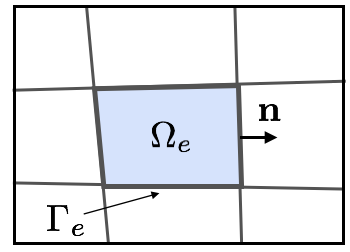
\includegraphics[width=1.5in]{DG_domain.png}
\label{fig:spatial_discretization/dg_domain}}
\subfigure[Element $\Omega_e$]{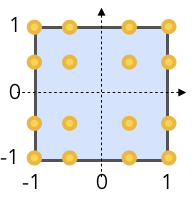
\includegraphics[width=1.5in]{DG_element.png}
\label{fig:spatial_discretization/dg_element}}
\end{center}
\caption{The (a) global domain and (b) element ($N=3$) for the DG method.}
\label{fig:spatial_discretization/dg_method}
\end{figure}

To construct discrete approximations of continuous differential operators (e.g., gradient, divergence, or curl) with the DG method, we first must represent the solution vector (call it $q$) using a polynomial representation.  That is, we represent the solution vector inside of each element $\Omega_e$ as follows
\be
q^{(e)}_N(\vc{x},t) = \sum_{i=1}^{M_N} \psi_i(\vc{x}) q^{(e)}_i(t)
\label{eq:spatial_discretization/dg_method}
\ee
where $\psi(\vc{x})$ are the known basis functions and $q^{(e)}_i(t)$ is the solution at each degree of freedom which will be time-dependent.
The superscript $(e)$ represents the specific element we are working with, $i=1,\ldots,M_N$ represents degrees of freedom inside each element $\Omega_e$.  Figure \ref{fig:spatial_discretization/dg_domain} shows a sample global domain whereby we then identify one specific element $\Omega_e$ to work with.  We then map the element from its physical space to the reference element presented in Fig.\ \ref{fig:spatial_discretization/dg_element}; in this particular example $M_N=(N+1)^2$ where $N=3$ which means we are using 3rd degree polynomials in each direction (yielding 4th degree accuracy).  In general, $N$ need not be constant in each direction and so we can also write $M_N=(N_{\xi}+1)(N_{\eta}+1)$ in two dimensions or $M_N=(N_{\xi}+1)(N_{\eta}+1)(N_{\zeta}+1)$ in three dimensions, where $\xi$ is along the horizontal direction, $\eta$ along the vertical, and $\zeta$ coming out of the page. 

The attraction of using basis functions $\psi$ to represent the solution $q$ is that computing the gradient of $q$ now only requires applying the gradient operator directly to Eq.\ \eqref{eq:spatial_discretization/dg_method} which yields
\be
\nabla q^{(e)}_N(\vc{x},t) = \sum_{i=1}^{M_N} \nabla \psi_i(\vc{x}) q^{(e)}_i(t)
\label{eq:spatial_discretization/dg_method/gradient}
\ee
where we are able to construct $\grad \psi$ \emph{a priori} since we have chose $\psi$ and these basis functions do not change in time (unless p-refinement is used which we will not consider here).

\subsubsection{DG Representation of Conservation Laws}
To describe the DG method, let us use it to represent the divergence operator for the conservation law
\be
\diff{q}{t} + \nabla \cdot \vc{f} = 0
\label{eq:spatial_discretization/DG_divergence/conservation_law}
\ee
where, in two dimensions, $f$ has components $\vc{f}=f_x \wh{\vc{i}} + f_y \wh{\vc{j}}$.
To construct a discrete approximation to Eq.\ \eqref{eq:spatial_discretization/DG_divergence/conservation_law} we first multiply by a test function $\psi_i$ and integrate within each element $\Omega_e$ as follows
\be
\inte \psi_i \diff{q^{(e)}_N}{t} d\Omega_e + \inte \psi_i \nabla \cdot \vc{f}^{(e)}_N d\Omega_e= 0.
\label{eq:spatial_discretization/DG_divergence/conservation_law/discrete}
\ee
Using the product rule, the second term can be written as follows
\be
\inte \psi_i \diff{q^{(e)}_N}{t} d\Omega_e + \inte \nabla \cdot \left( \psi_i \vc{f}^{(e)}_N \right) d\Omega_e - \inte \nabla \psi_i \cdot \vc{f}^{(e)}_N d\Omega_e= 0
\label{eq:spatial_discretization/DG_divergence/conservation_law/discrete2}
\ee
and invoking the divergence theorem for the second term yields
\be
\inte \psi_i \diff{q^{(e)}_N}{t} d\Omega_e + \intb \psi_i \nvector \cdot \vc{f}^{(e)}_N d\Gamma_e - \inte \nabla \psi_i \cdot \vc{f}^{(e)}_N d\Omega_e= 0
\label{eq:spatial_discretization/DG_divergence/conservation_law/discrete3}
\ee
where $\Gamma_e$ is the boundary of the element $\Omega_e$ and $\nvector$ is its outward pointing normal vector. We now need to fix the inconsistency of the second term above because it says that the solution along each element boundary $\Gamma_e$ is different from its neighbor since $\vc{f}^{(e)}_N$ is allowed to be discontinuous across element boundaries.  To fix this, we introduce a numerical flux such that what flows from element $\Omega_e$ to its neighbor $\Omega_k$ is the negative of what flows from $\Omega_k$ into $\Omega_e$.  We represent this fix as follows
\be
\inte \psi_i \diff{q^{(e)}_N}{t} d\Omega_e + \intb \psi_i \nvector \cdot \vc{f}^{(*,e)}_N d\Gamma_e - \inte \nabla \psi_i \cdot \vc{f}^{(e)}_N d\Omega_e= 0
\label{eq:spatial_discretization/DG_divergence/conservation_law/discrete4}
\ee
where $\vc{f}^{(*,e)}_N$ is the numerical flux that takes into account the solution at $\Omega_e$ and all its neighbors $\Omega_k$ represented by $\Gamma_e$.  In two dimensions we will have 4 face neighbors and in three dimensions we will have 6 face neighbors.  At this point one is free to choose their favorite numerical flux $\vc{f}^{(*,e)}_N$ just as one would do in the finite volume method (e.g., Rusanov, Roe, HLL, HLLC, etc.).  Note that it is the numerical flux term that couples all of the equations together; the rest of the terms are purely local within the element - this should be quite familiar for those of you coming from the finite volume community.

\subsubsection{Tensor Product Basis Functions}
In Eq.\ \eqref{eq:spatial_discretization/dg_method} we have said very little about the basis functions $\psi$ and have written the approximation in so-called monolithic form whereby all the degrees of freedom within an element are written as one long vector of length $M_N$.  This way of representing Eq.\ \eqref{eq:spatial_discretization/dg_method} allows for a quick explanation of the DG method but does not illustrate how the method is constructed when tensor product basis functions are used which is what we propose here.  In the case of tensor product basis functions, we rewrite $\psi$ (in 2D) as follows
\[
\psi_i(\xi,\eta) = h_j(\xi) \otimes h_k(\eta)
\]
where $h$ are one-dimensional basis functions, and $\otimes$ denotes the tensor (or Kronecker) product, and $j=1,\ldots N_{\xi}+1$, $k=1,\ldots,N_{\eta}+1$, and $i=j + (k-1) \left( N_{\xi}+1 \right)$. Using this strategy we can now rewrite Eq.\ \eqref{eq:spatial_discretization/dg_method} as follows
\be
q^{(e)}_N(\xi,\eta,t) = \sum_{i=1}^{N_{\xi}+1} \sum_{j=1}^{N_{\eta}+1} h_i(\xi) h_j(\eta) q^{(e)}_{ij}(t)
\label{eq:spatial_discretization/dg_method/tensor-product}
\ee
where we have written the approximation in terms of the reference element coordinates $(\xi,\eta$ instead of the physical coordinates $(x,y)$.  The advantage of doing this is that the reference element and its coordinates never change (assuming no p-refinement) which means that we can use one set of basis functions for all of the elements in the mesh.  

Taking the gradient of Eq.\ \eqref{eq:spatial_discretization/dg_method/tensor-product} yields
\be
\diff{}{\vc{x}} q^{(e)}_N(\xi,\eta,t) = \diff{}{\vc{x}} \sum_{i=1}^{N_{\xi}+1} \sum_{j=1}^{N_{\eta}+1} h_i(\xi) h_j(\eta) q^{(e)}_{ij}(t)
\label{eq:spatial_discretization/dg_method/tensor-product/gradient}
\ee
where $\vc{x}$ can represent either $x$ or $y$.  Let us look at each component separate and so invoking the chain rule yields
\[
\diff{}{x}=\diff{}{\xi} \diff{\xi}{x} + \diff{}{\eta} \diff{\eta}{x}
\]
and
\[
\diff{}{y}=\diff{}{\xi} \diff{\xi}{y} + \diff{}{\eta} \diff{\eta}{y}
\]
where the metric terms $\diff{\vc{\xi}}{\vc{x}}$ need to be computed for each element in the mesh.
Using these we can now rewrite Eq.\ \eqref{eq:spatial_discretization/dg_method/tensor-product/gradient} for the x-derivative as follows
\be
\diff{}{x} q^{(e)}_N(\xi,\eta,t) = \sum_{i=1}^{N_{\xi}+1} \sum_{j=1}^{N_{\eta}+1} \left( \diff{h_i(\xi)}{\xi}\diff{\xi}{x} h_j(\eta) + h_i(\xi) \diff{h_j(\eta)}{\eta}\diff{\eta}{x} \right) q^{(e)}_{ij}(t).
\label{eq:spatial_discretization/dg_method/tensor-product/x-deriv}
\ee
If we use the same polynomial order along $\xi$ and $\eta$ we can simplify Eq.\ \eqref{eq:spatial_discretization/dg_method/tensor-product/x-deriv} as follows
\be
\diff{}{x} q^{(e)}_N(\xi,\eta,t) = \sum_{i=1}^{N_{\xi}+1} \sum_{j=1}^{N_{\eta}+1} \left( dh_i \xi_x h_j + h_i dh_j \eta_x \right) q^{(e)}_{ij}(t).
\label{eq:spatial_discretization/dg_method/tensor-product/x-deriv2}
\ee
where $h$ is the basis function and $dh$ is its derivative, which are the same functions used along both directions $\xi$ and $\eta$; the index $(i,j)$ will account for which direction we are referring to.


\subsection{Time-Discretization Methods}

In order to circumvent the time-step restriction due to the fast moving acoustic waves, we will rely on implicit-explicit (IMEX) methods . For the LES model, if the aspect ratio of the horizontal to vertical grid spacing is near unity, it will be beneficial to use fully 3D-IMEX methods.  For the global atmospheric model, we propose to use 1D-IMEX methods whereby the time-integrator is fully explicit in the horizontal direction (HE) and implicit in the vertical direction (so-called HEVI schemes).

We propose to use a general family of additive Runge-Kutta methods (ARK) methods for both the 1D and 3D IMEX approaches (see, e.g., \cite{giraldo:2013} for 1D and 3D-IMEX methods based on ARKs). Note that adding fully-implicit Runge-Kutta (IRK) methods to the 3D-IMEX approach is quite trivial so this can be included as an option. Fully-implicit methods have no time-step restriction with respect to stability.

To get a sense of how the ARK approach works, let us partition the right-hand-side function $S(\vc{q})$ into its linear $L(\vc{q})$ and nonlinear $N(\vc{q})$ parts where the stiffness due to grid spacing or acoustic waves are contained in $L(\vc{q})$.  This then allow us to write the semi-discrete form (in space) as follows
\[
\diff{\qvector}{t} = L(\qvector) + N(\qvector) 
\]
which can now be discretized in time.  First we compute the stage values
\[
\vc{Q}^{(i+1)}=\qvector^n + \Delta t \sum_{k=0}^{i} \left( a_k N(\vc{Q}^{(k)}) \right) + \Delta t \sum_{k=0}^{i+1} \left( \wt{a}_k L(\vc{Q}^{(k)}) \right)
\]
with $i=0,\ldots,s$ where $s$ are the number of stages, $a$, and $\wt{a}$ are the coefficients of the double Butcher tableau defined in \cite{kennedy:2003,giraldo:2013}.  Additionally, 
$\vc{Q}^{(0)}=\qvector^n$ and the solution at time $n+1$ is obtained as follows
\[
\vc{q}^{n+1}=\qvector^n + \Delta t \sum_{k=0}^{s} \left( b_k S(\vc{Q}^{(k)}) \right)
\]
where the coefficients $b$ are also found in \cite{kennedy:2003,giraldo:2013}.
So far we have defined a diagonally-implicit Runge-Kutta (DIRK) method \cite{alexander:1977,butcher:1981a,ascher:1997,boscarino:2009}.  To make the DIRK more efficient, we impose the restriction that all the diagonal values $\wt{a}_{ii}$ to be constant. This allows one construction of the matrix problem which does not change across stage values.  This we now refer to as singly-diagonally-implicit Runge-Kutta (SDIRK).


\section{Sub-grid Scale Models}
\label{sec:sgs_models}

In order to discuss the sub-grid scale models required for the nonhydrostatic atmospheric models, let us write the equations in the following compact form  
\[
\diff{\vc{q}}{t} = S_D(\vc{q}) + S_P(\vc{q})
\]
where $\vc{q}$ is the solution vector, $S_D$ denotes the RHS due to the dry dynamics while $S_P$ denotes the RHS due to the moist physics. We have already described $S_D$ so let us now focus on $S_P$.

\subsection{Moist Physics}
In MLAM, we propose to use a simplified moisture process (e.g., warm rain Kessler physics) with a Lilly-Smagorinsky type mixing scheme.    (Do we need long-wave radiation? Other such schemes?  If so, which ones?)

\subsection{Topography}
Will be incorporated at a later date.

\section{Computing Aspects}
\label{sec:computing_aspects}

Let us decompose the computing aspects into the following groups
\begin{enumerate}
\item workflow language
\item parallelization API
\item many-core API
\item graph-partitioning and grid generation

\end{enumerate}

\subsection{Workflow Language}
Although Python is a popular workflow language, we will likely explore Julia as another option.  The reasons for possibly using Julia are: 
\begin{itemize}
\item We would like to use one language for both prototyping and workflow development,
\item Unlike Python, Julia was built for high-performance computing (see Sec.\ \ref{sec:computing_aspects/manycore}),
\item If we engage with the Julia community, we can get many good students to participate in various forms,
\item Risk-mitigation plan includes falling back to pure C code with Python scaffolding and OCCA kernels.
\end{itemize} 

\subsection{Parallelization API}
We propose to use the Message-Passing Interface (MPI) for communicating across processors and nodes (with multiple processors).  One of the NPS team members (Lucas Wilcox) has written Julia wrappers for MPI.

\subsection{Many-core API}
\label{sec:computing_aspects/manycore}
We propose to use a GPU library for accessing the GPUs. The NPS team has vast experience in this area. For example, the NPS team ported NUMA using OCCA2 with a CUDA back-end to run on the Titan supercomputer using 16,000 GPU cards achieving very good weak scaling (see \cite{abdi:2016b,abdi:2018}). The approach will be to write all of the compute-kernels in either GPUArrays (from Julia), OCCA2, or CUDA. From our perspective, the compute-kernel is the focus and most GPU-ready kernels look more or less the same (OCCA, CUDA, and OpenCL). 

\subsection{Graph-Partitioning and Grid Generation}
One of the NPS team members (Jeremy Kozdon) has written Julia wrappers to the p4est library developed by another NPS team member (Lucas Wilcox).  We propose to use p4est for both grid-generation and graph-partitioning or Metis with a specific grid generator for both the LES and global domains. The global domain will use a cubed-sphere grid while the LES domains will use a logically Cartesian cube grid.

\subsection{Code-base Repository}
The code is maintained in Github at \url{https://github.com/climate-machine}

\subsection{Software Management}
Software engineers are required in order to maintain the coupled software-base and to have a centralized person "in charge" of the software code.  It could also be helpful to have a support person who can dedicate time to help with HPC issues on running on the specific Caltech cluster that we will use.  

\subsection{Computing Hardware}
We propose to use about \$30K for purchasing a number of GPU cards.  Most of the development work will be performed on this new GPU cluster at NPS.  We will also  time available to us on the Caltech cluster. We also need to consider which types of computers we will be targeting (e.g., Summit at ORNL) although this will not happen until after year 1.


\section{Machine Learning}
\label{sec:machine_learning}

In this section, we shall describe the role of the non-hydrostatic atmospheric models in the machine learning/data assimilation approach.  To make the exposition clear, let us represent the model in the following way
\[
\diff{\vc{q}}{t} = S_C(\vc{q}) + S_{NC}(\vc{q})
\]
where $\vc{q}$ is the solution vector, $S_C$ denotes the computable terms on the RHS of the equations while $S_{NC}$ denotes the non-computable parameters.  Examples of computable terms includes the full dry dynamics in addition to explicit convection.  Non-computable terms are those that are below the sub-grid scales of even an LES model.  These terms will be obtained from observational data.  Let us describe the nature of this data and how often it needs to be read in.

\subsection{Non-computable Terms}
What sort of data will we be reading in and how often? Once per simulation?  

\subsection{LES Model}
The LES model will require approximately 1 million DOF.  We are targeting 10-100 meter resolutions at this range.

\subsection{Global Model}
Need to describe the process of how to spin-off the LES models and use them to improve the global model. 200 km global resolutions or better if we can afford it. 


%-------Bibliography
\bibliographystyle{siam}
\bibliography{Giraldo_refs}

\end{document}
